% !TEX encoding = UTF-8
% !TEX TS-program = pdflatex
% !TEX root = ../../tesi.tex

\section{Lo standard ERC721 per Hotmoka}
Dato che Hotmoka è una \textit{blockchain} ancora giovane è risultata necessaria lo sviluppo dello standard ERC721 per Hotmoka, dato che non ne ha uno.

\subsection{Progettazione}
Per quanto riguarda la progettazione dello standard ERC721 per Hotmoka, ho preso ispirazione dall'implementazione realizzata dall'azienda OpenZeppelin che lo ha sviluppato per Ethereum.

Non l'ho scritto tutto, ma solamente determinate componenti che risultavano necessarie per l'implementazione successiva del contratto per la gestione degli NFT.

I \textit{design pattern} utilizzati sono solamente il \textbf{\textit{Guard Check}}.

Per aiutarmi e poter realizzare un'architettura complicata come quella dello standard ERC721, ho preso spunto anche dall'implementazione, già realizzata, dello standard ERC20 (standard che gestisce i \textit{token} fungibili in Ethereum) in Takamaka.

\clearpage
\begin{figure}
  \centering
  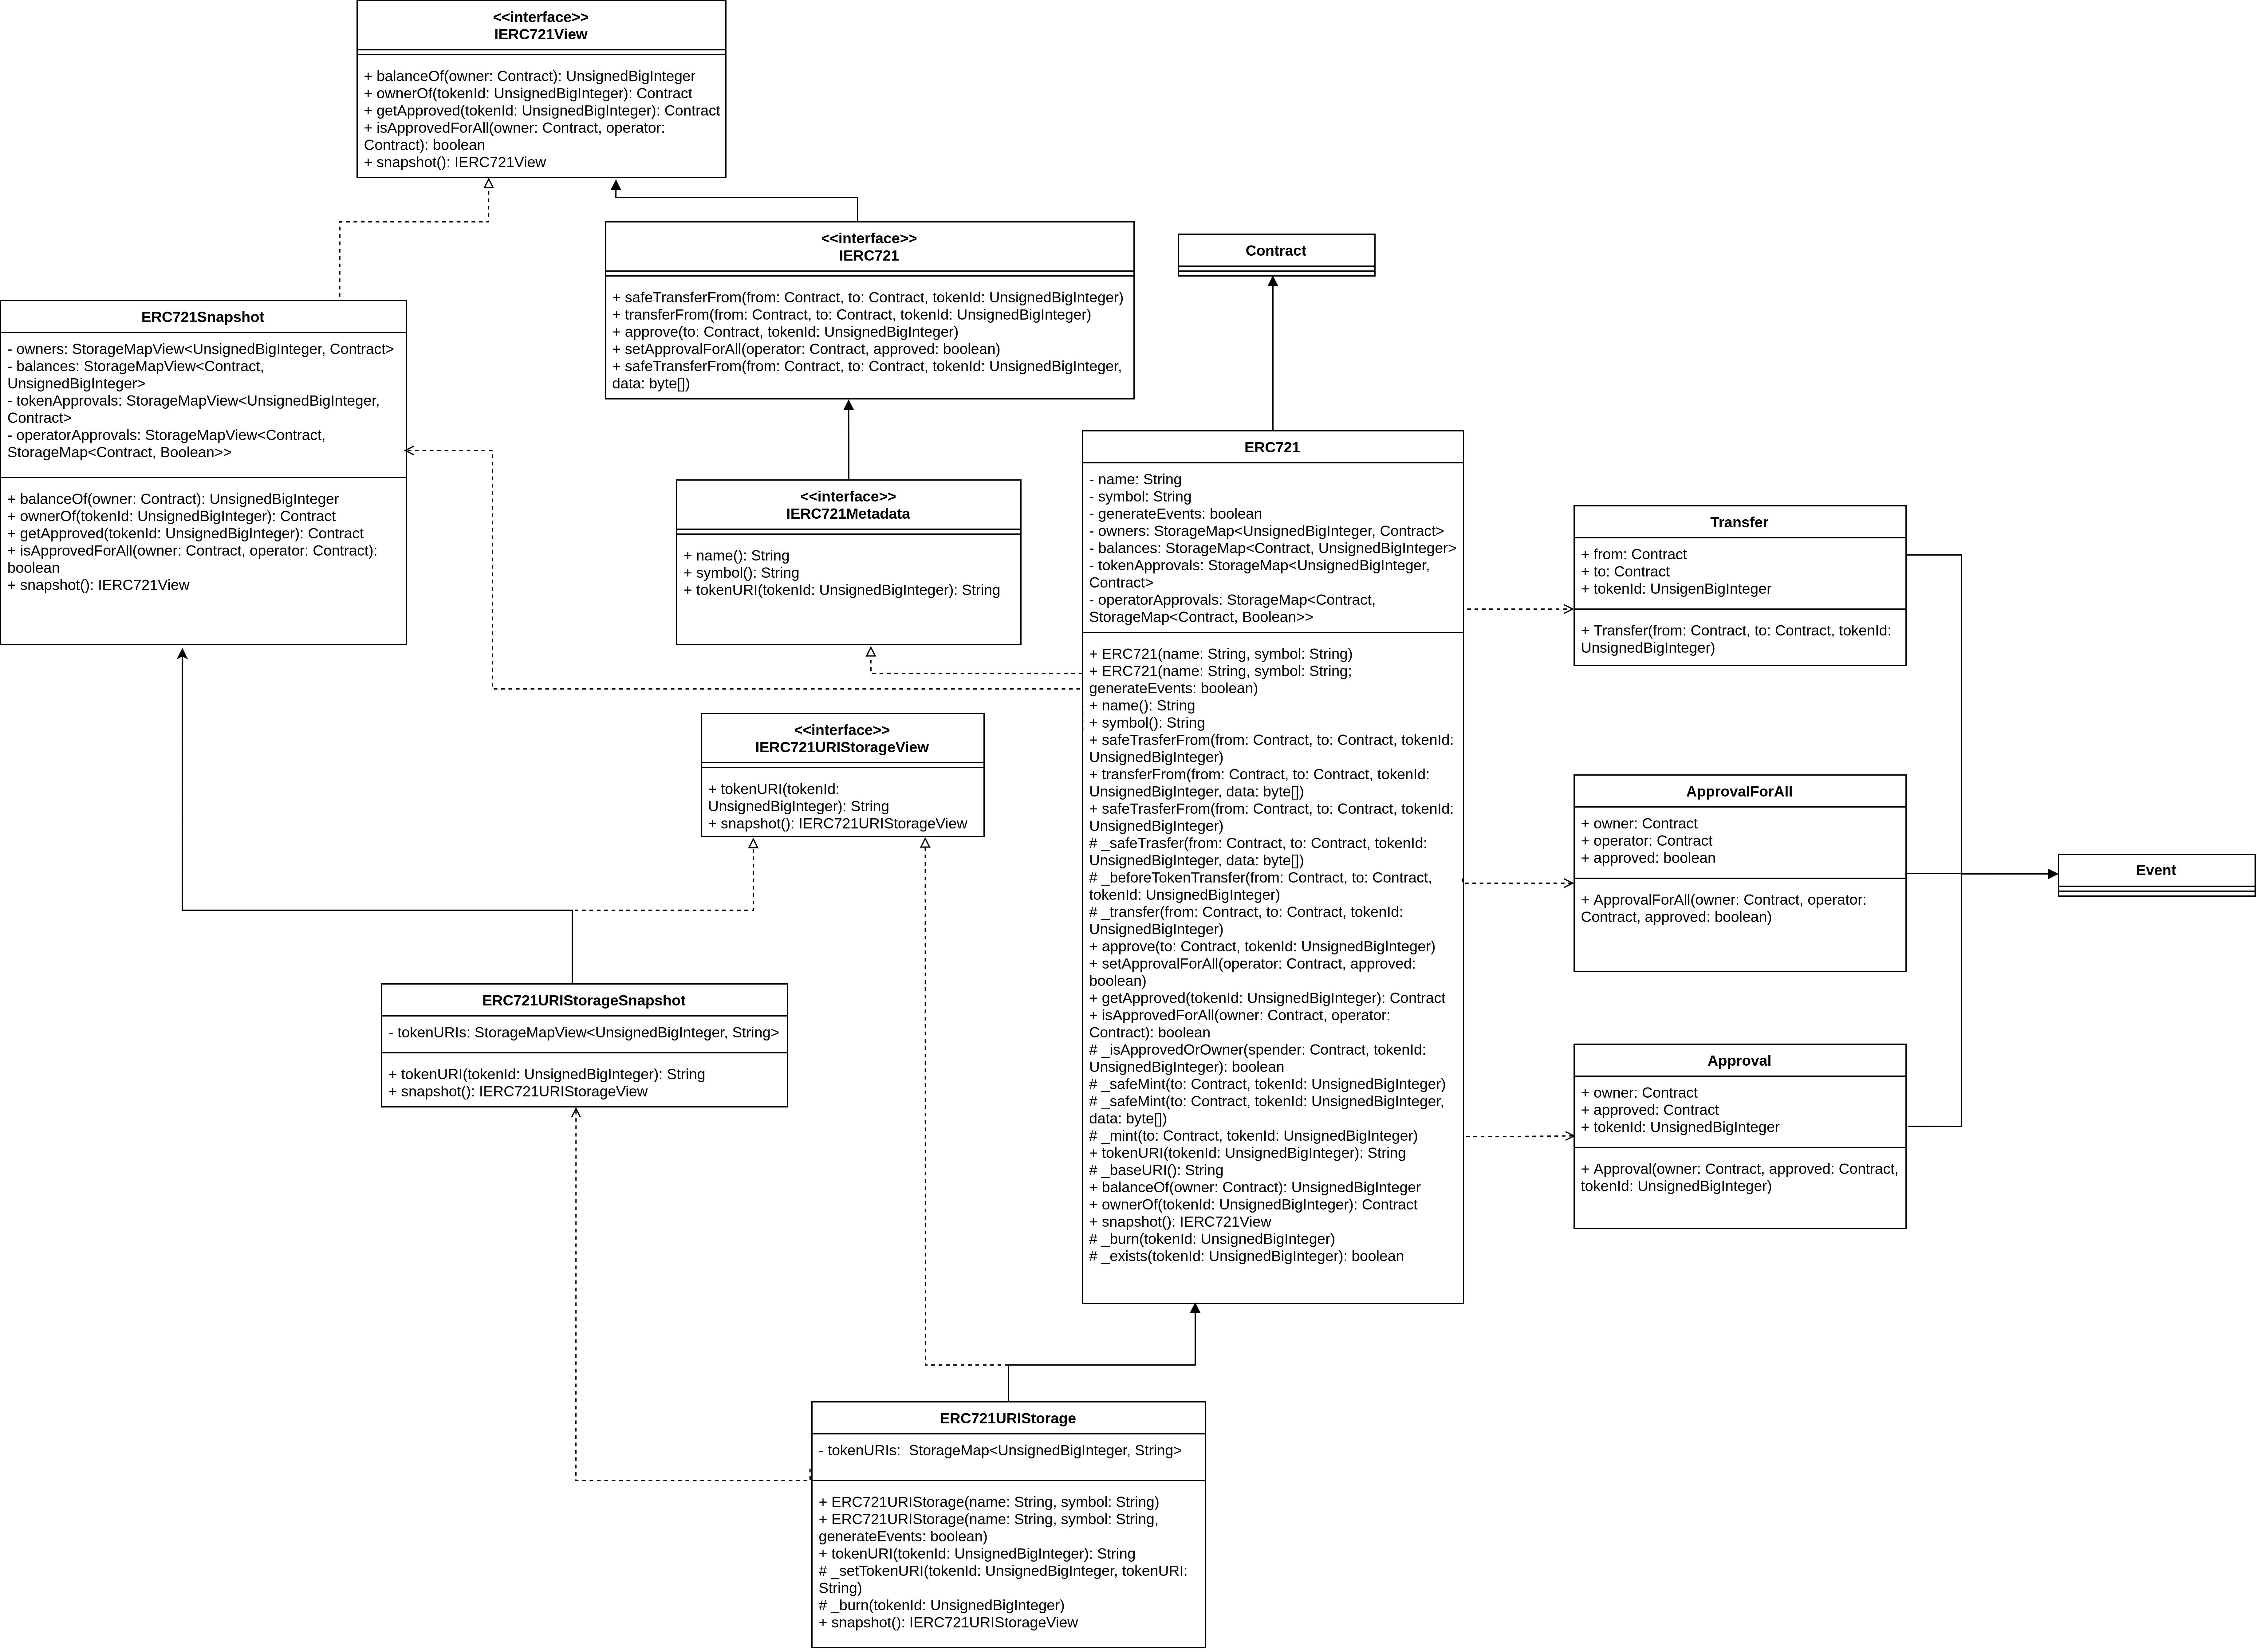
\includegraphics[width=\textwidth]{capitolo3/class-diagram/erc721-hotmoka-class-diagram.png}
  \caption{Diagramma delle classi dell'implementazione dello standard ERC721 per Hotmoka}
  \label{fig:erc721-hotmoka-class-diagram}
\end{figure}

Come si può vedere in dal diagramma delle classi (figura \ref{fig:erc721-hotmoka-class-diagram}) per permettere l'esecuzione dello \textit{Snapshot} dello stato attuale della \textit{blockchain}, sono state dichiarate delle interfacce separate che racchiudono solo le funzioni che sono targate \textit{view}. In questo modo chiunque potrà eseguire quelle funzioni in una copia dello stato attuale della rete, senza avere inconsistenze.

\subsection{Codifica}
In seguito alla fase di progettazione, sono passato alla codifica. Anche qui ho prima scritto tutta la struttura di quanto dovevo sviluppare, ovvero classi e firme, ed in seguito sono passato alla scrittura del corpo. \\

\clearpage

\begin{figure}[h!]
  \centering
  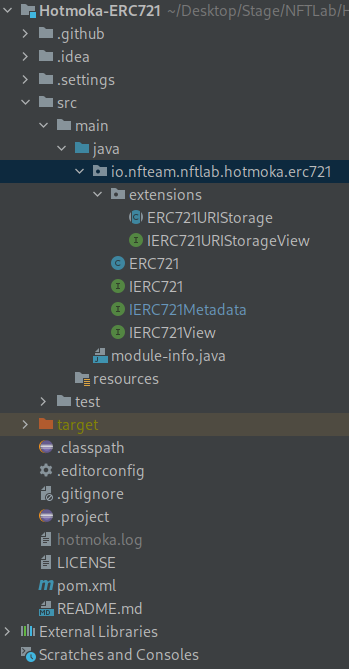
\includegraphics[width=0.3\textwidth]{capitolo3/erc721-hotmoka/erc721-hotmoka-structure.png}
  \caption{Struttura del progetto dello standard ERC721 per Hotmoka}
\end{figure}

Meritevole di attenzione è l'implementazione del sistema dello \textit{Snapshot}.

\clearpage

\begin{figure}[h!]
  \centering
  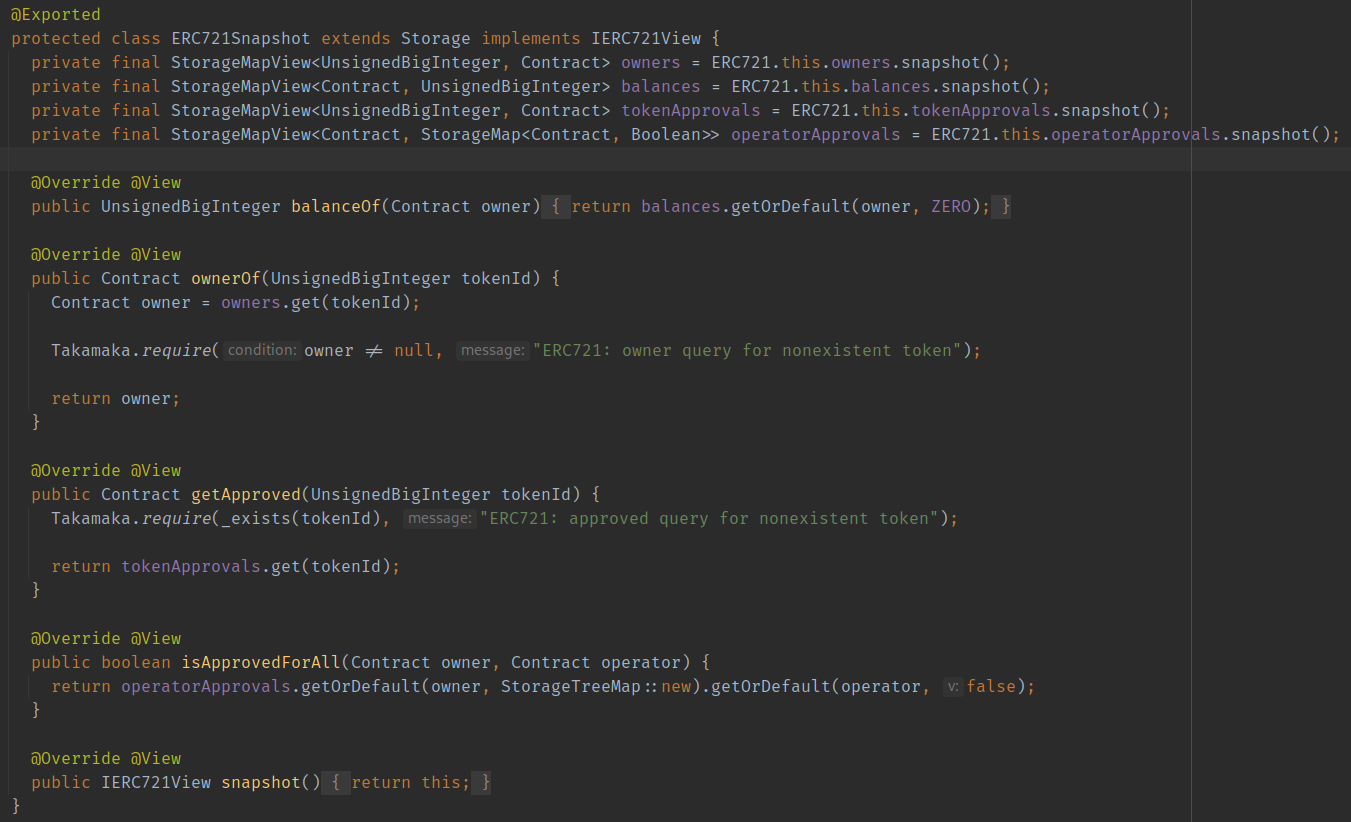
\includegraphics[width=0.8\textwidth]{capitolo3/erc721-hotmoka/erc721-hotmoka-snapshot.png}
  \caption{Implementazione del sistema dello \textit{Snapshot} di un oggetto di tipo ERC721}
  \label{fig:erc721-snapshot}
\end{figure}

Come si può vedere in figura \ref{fig:erc721-snapshot} viene eseguito lo \textit{snapshot} dello stato attuale e vengono implementati i metodi per leggerlo.

\subsection{Verifica}
Per quanto concerne la verifica dello standard ERC721 per Hotmoka, dopo una discussione con il mio \textit{tutor} aziendale Fabio Pallaro, è stato deciso che non c'è il bisogno di verificare attraverso la scrittura di test automatici, anche questa parte del progetto. La seguente scelta è stata presa perché, inizialmente non era prevista la scrittura dello standard ERC721 per Hotmoka. In più non c'era abbastanza tempo per poterli implementare.
